\documentclass[a4paper,12pt]{article}

% Import the deliverable package from common directory
\usepackage{../common/deliverable}

\usepackage{beamerarticle}
%%\documentclass[ignorenonframetext,red]{beamer}

%\mode<article>{\usepackage{fullpage}}
\mode<presentation>{\usetheme{RomaTorVergata}}
% Tell LaTeX where to find graphics files
\graphicspath{{../common/logos/}{./figures/}{../}}

\usepackage{xspace}


% Set the deliverable number (without the D prefix, it's added automatically)
\setdeliverableNumber{1.6}
% Various utilities for the slides.

%\usepackage[utf8x]{inputenc}
%\usepackage[T1]{fontenc}

\usepackage{listings}
\lstset{basicstyle=\ttfamily,
	showstringspaces=false,
	commentstyle=\color{red},
	keywordstyle=\color{blue},
	emph={%  
		psb_init, psb_info, psb_exit,%
		psb_get_mpi_comm,psb_get_mpi_rank,%
		psb_snd,psb_rcv,%
		psb_bcast,
		psb_sum,
		psb_amx,
		psb_amn,
		psb_max,
		psb_min,
                psb_scan_sum,
                psb_exscan_sum,
		psb_geaxpby,
		psb_spmm,
		psb_gedot,
		psb_genrm2,
		psb_halo,
		psb_cdall,
		psb_sum,
		psb_cdins,
		psb_cdasb,
		psb_spall,
		psb_spins,
		psb_spasb,
		psb_sprn,
		psb_sp_clone,
		psb_geall,
		psb_geins,
		psb_geasb,
		psb_glob_to_loc,
		psb_loc_to_glob,
		psb_krylov,
		psb_precinit,
		psb_precbld,
		psb_geamax,
		psb_geasum,
		psb_spnrmi,
		psb_spsm,
		mm_array_write,
		mm_mat_write,
		mm_array_read,
		mm_mat_read,
		hb_read,
		hb_write,
		init,
		set,
		hierarchy_build,
		smoothers_build,
		build,
		cscnv,
		apply,
		free,
		descr,
                mode,
                request
	},emphstyle={\color[HTML]{E4605B}}%
}

\definecolor{keycolor}{RGB}{172, 42, 42}
\definecolor{mbleu}{RGB}{64,96,127}
\definecolor{vimvert}{RGB}{46, 139, 87}
\definecolor{Red}{rgb}{1.0, 0.01, 0.24}
\definecolor{Lime}{rgb}{0.75, 1.0, 0.0}
\definecolor{Yellow}{rgb}{1.0, 0.77, 0.05}
\definecolor{gray}{rgb}{0.66, 0.66, 0.66}
\definecolor{ao(english)}{rgb}{0.0, 0.5, 0.0}
\definecolor{codecolor}{HTML}{eae1de}
\definecolor{ttqqqq}{rgb}{0.2,0,0}

\def\zz{\color{mbleu}\textless\bgroup\itshape\aftergroup\endzz}
\def\endzz{\textgreater\egroup}

\lstdefinestyle{global}{
	basicstyle=\ttfamily\scriptsize\color{black!90},%
	stringstyle=\itshape\color{magenta},%
	showstringspaces=false,%
	keywordstyle=\bfseries\color{keycolor},%
	commentstyle=\color{blue}\slshape,%
	framexleftmargin=1mm,%
}

\lstdefinestyle{makefile}{
	otherkeywords={.SUFFIXES},
	morekeywords={SUFFIX, CPP_,},
	moredelim=[is][\color{mbleu}]{/*}{*/},
	style=global,%
	morecomment=[l][commentstyle]{\#},%
	emphstyle={\color{vimvert}},%
	moredelim=[s][\color{vimvert}]{\$(}{)}%
}
\def\bx{{\mathbf x}}
\def\bb{{\mathbf b}}
\def\br{{\mathbf r}}
\def\be{{\mathbf e}}
\def\bK{{\mathbf K}}
\def\bu{{\mathbf u}}
\def\bw{{\mathbf w}}
\newcommand{\R}{{\mathcal R}}
\newcommand{\Range}{{\mathcal Range}}
\usepackage{bbding}
\usepackage{fontawesome5}

\usepackage{multicol}
\usepackage{pgfplots}
\usepackage{pgfkeys}
\usepackage{tikz}
\usetikzlibrary{chains,shapes.arrows,shapes.multipart,
  arrows,arrows.meta,positioning,decorations,,
  decorations.pathreplacing,matrix,
  decorations.pathmorphing,plothandlers}
\tikzset{
    >=stealth',
    punktchain/.style={
        rectangle, 
        rounded corners, 
        % fill=black!10,
        draw=white, very thick,
        text width=6em,
        minimum height=2em, 
        text centered, 
        on chain
      }
    }
\usepackage{pgf-pie}
\usepackage{amsmath,amssymb,amsfonts}
\usepackage{smartdiagram}
\usepackage{natbib}
\usepackage[tworuled,linesnumbered]{algorithm2e}
\usepackage{colortbl}%
\newcommand{\myrowcolour}{\rowcolor[gray]{0.925}}
\usepackage{booktabs}

%\usepackage{pgfpages}
\usepackage{pgfmorepages}
\pgfmorepagesloadextralayouts


\newcommand*{\tred}[1]{\textcolor{red}{#1}}
\newcommand*{\tgreen}[1]{\textcolor{green}{#1}}
\newcommand*{\tblu}[1]{\textcolor{blue}{#1}}
% Begin document
\begin{document}
\pgfpagesuselayout{1 on 1}[a4paper]
% Create the title page with the title as argument
\maketitlepage{Tutorials based on external libraries}

\newpage

% Main Table using the new environment and command
\begin{deliverableTable}
    \tableEntry{Deliverable title}{Tutorials based on external libraries}
    \tableEntry{Deliverable number}{D1.6}
    \tableEntry{Deliverable version}{0.1}
    \tableEntry{Date of delivery}{Feb 28th 2026}
    \tableEntry{Actual date of delivery}{[Actual date]}
    \tableEntry{Nature of deliverable}{Report/etc.]}
    \tableEntry{Dissemination level}{Public}
    \tableEntry{Work Package}{WP1}
    \tableEntry{Partner responsible}{UNITOV}
\end{deliverableTable}

% Abstract and Keywords Section
\begin{deliverableTable}
    \tableEntry{Abstract}{This report contains the tutorial on the
      external library PSCToolkit, delivered to the dealii-X project
      during the winter school event at SISSA on Dec. 11th and 12th, 2025.}
    \tableEntry{Keywords}{Linear algebra solvers. Libraries. Data
      structures.}
\end{deliverableTable}

\newpage

\begin{documentControl}
    \addVersion{0.1}{Feb 15th 2026}{Salvatore Filippone}{Initial draft}
    %\addVersion{0.2}{[Date]}{[Author name]}{[Description of changes]}
    %\addVersion{0.3}{[Date]}{[Author name]}{[Description of changes]}
    %\addVersion{1.0}{[Date]}{[Author name]}{Final version}
\end{documentControl}

\subsection*{{Approval Details}}
Approved by: [Name] \\
Approval Date: [Date]

\subsection*{{Distribution List}}
\begin{itemize}
    \item [] - Project Coordinators (PCs)
    \item [] - Work Package Leaders (WPLs)
    \item [] - Steering Committee (SC)
    \item [] - European Commission (EC)
\end{itemize}

\vspace*{2cm}

\disclaimer

\newpage

\tableofcontents % Automatically generated and hyperlinked Table of Contents

\newpage

\section{{Introduction}}

Work Package 1 is dedicated to the numerical software backbone of 
dealii-X, enabling the transition to exascale computing. One key
aspect of the WP is the interfacing with external libraries,
especially PSCToolkit~\url{https://psctoolkit.github.io} and MUMPS.
This interface is mostly transparent to the application end-user;
however, the developers need to acquire a working knowledge of the
features available and of the performance that can be attained. 

\subsection{{Purpose of the Document}}
The purpose of this document is to make available in deliverable
format the tutorial presentations given at the dealii-X winter school. 

\subsection{{Structure of the Document}}
\begin{itemize}
    \item Section \ref{sec:section2}: [Section Title]
    \item Section \ref{sec:section3}: [Section Title]
    \item Section \ref{sec:section4}: [Section Title]
    \item Section \ref{sec:section5}: [Section Title]
    \item Section \ref{sec:section6}: [Section Title]
\end{itemize}

\newpage

\section{PSCToolkit: PSBLAS 3.9 \& AMG4PSBLAS 1.2 Tutorial}
\label{sec:section2}
\begin{center}
  
\includegraphics[width=.95\textwidth]{tutorial-001.eps}\\[2\baselineskip]
  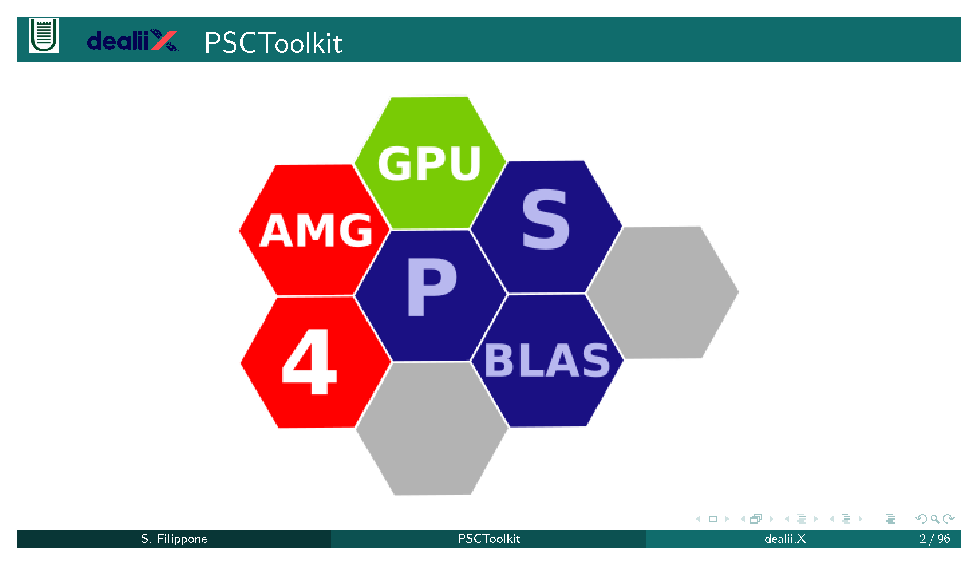
\includegraphics[width=.95\textwidth]{tutorial-002.eps}
\end{center}
\newpage
\begin{center}
  \includegraphics[width=.95\textwidth]{tutorial-003.eps}\\[2\baselineskip]
  
\includegraphics[width=.95\textwidth]{tutorial-004.eps}
\end{center}
\newpage
\begin{center}
  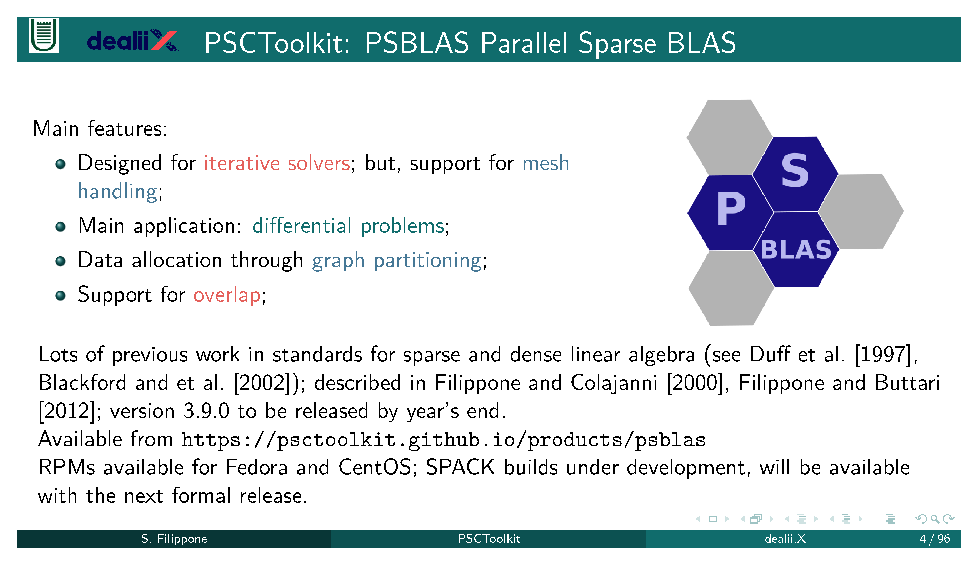
\includegraphics[width=.95\textwidth]{tutorial-005.eps}\\[2\baselineskip]
  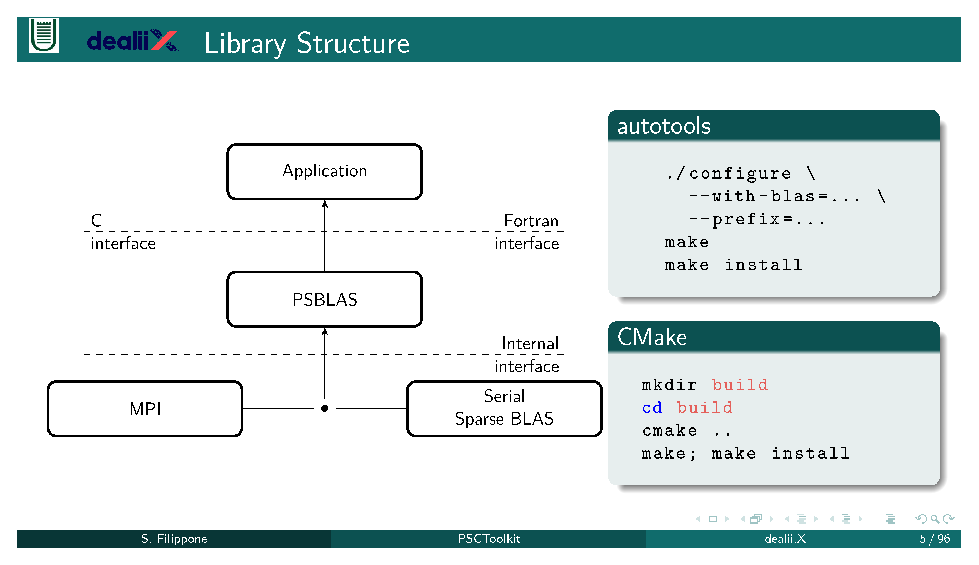
\includegraphics[width=.95\textwidth]{tutorial-006.eps}
\end{center}
\newpage
\begin{center}
  
\includegraphics[width=.95\textwidth]{tutorial-007.eps}\\[2\baselineskip]
  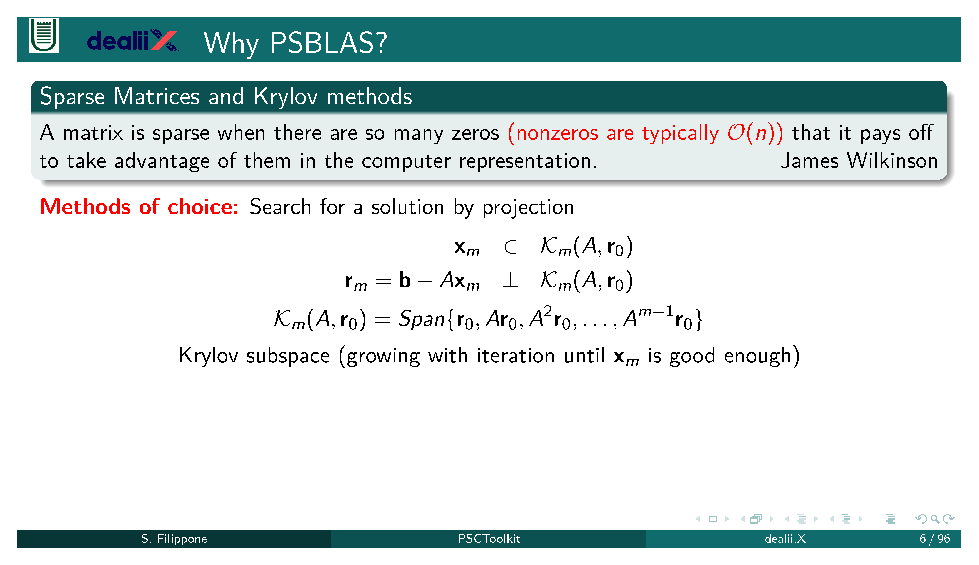
\includegraphics[width=.95\textwidth]{tutorial-008.eps}
\end{center}
\newpage
\begin{center}
  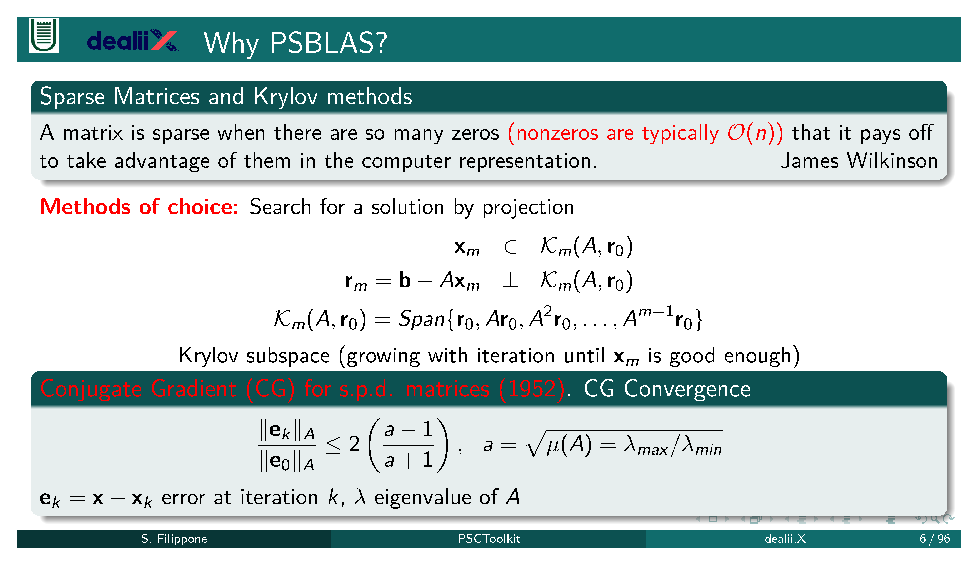
\includegraphics[width=.95\textwidth]{tutorial-009.eps}\\[2\baselineskip]
  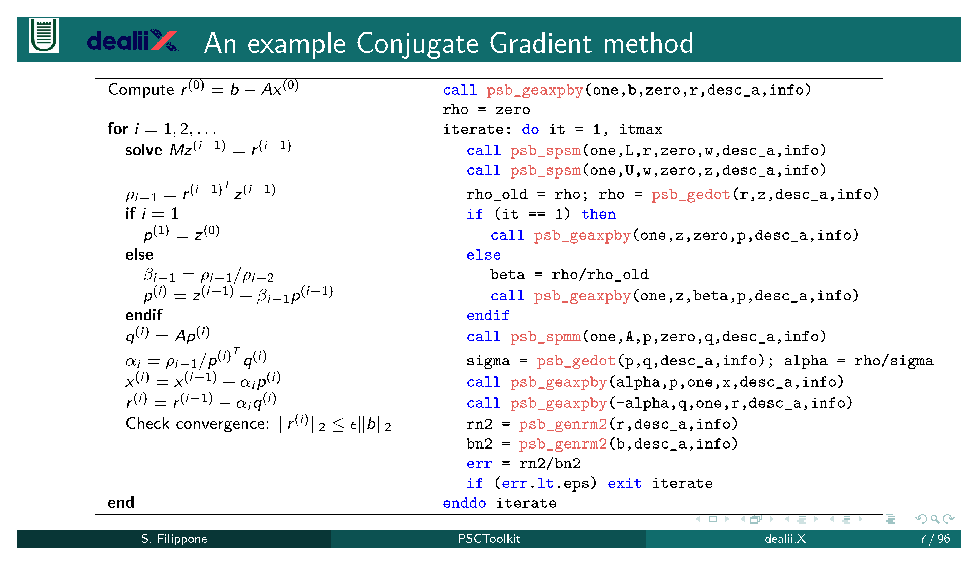
\includegraphics[width=.95\textwidth]{tutorial-010.eps}
\end{center}
\newpage
\begin{center}
  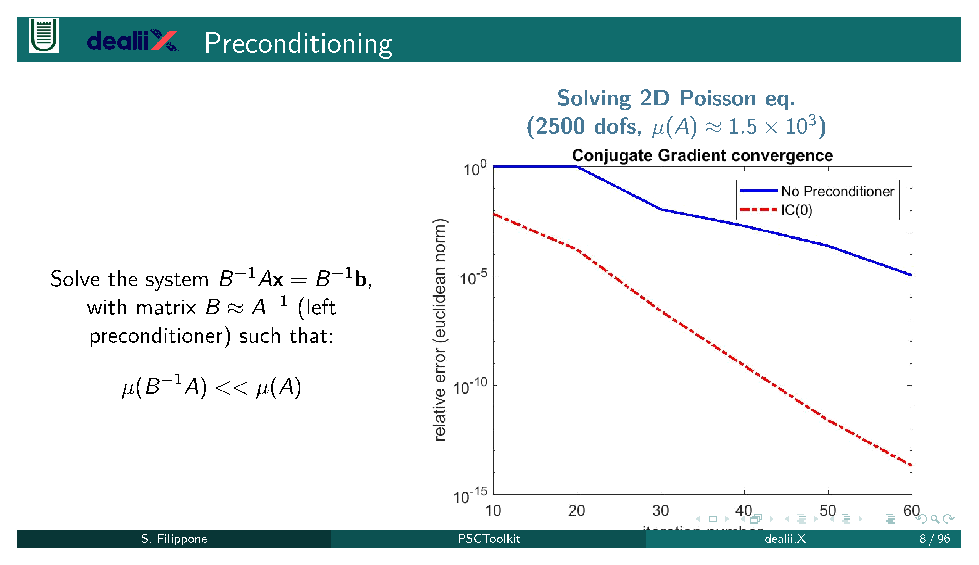
\includegraphics[width=.95\textwidth]{tutorial-011.eps}\\[2\baselineskip]
  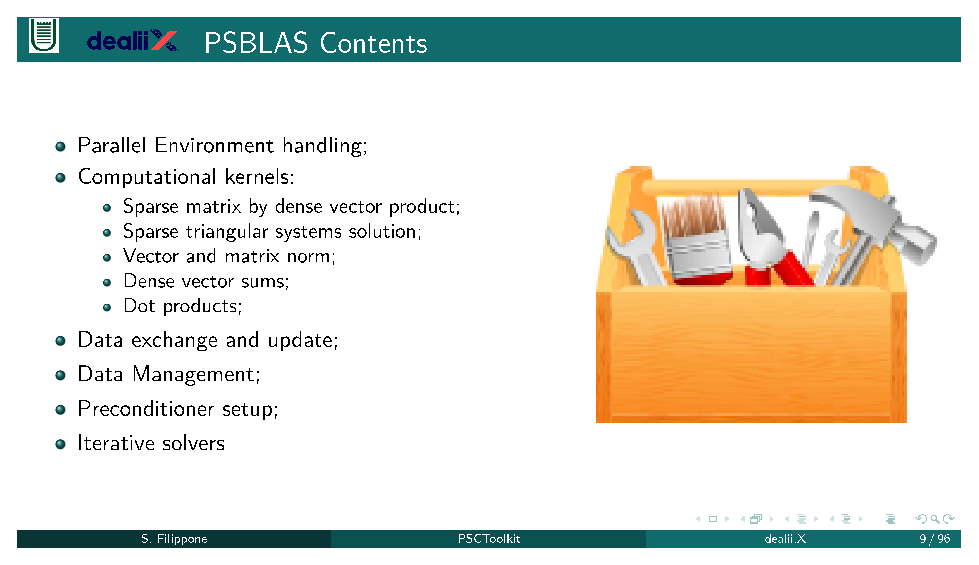
\includegraphics[width=.95\textwidth]{tutorial-012.eps}
\end{center}
\newpage
\begin{center}
  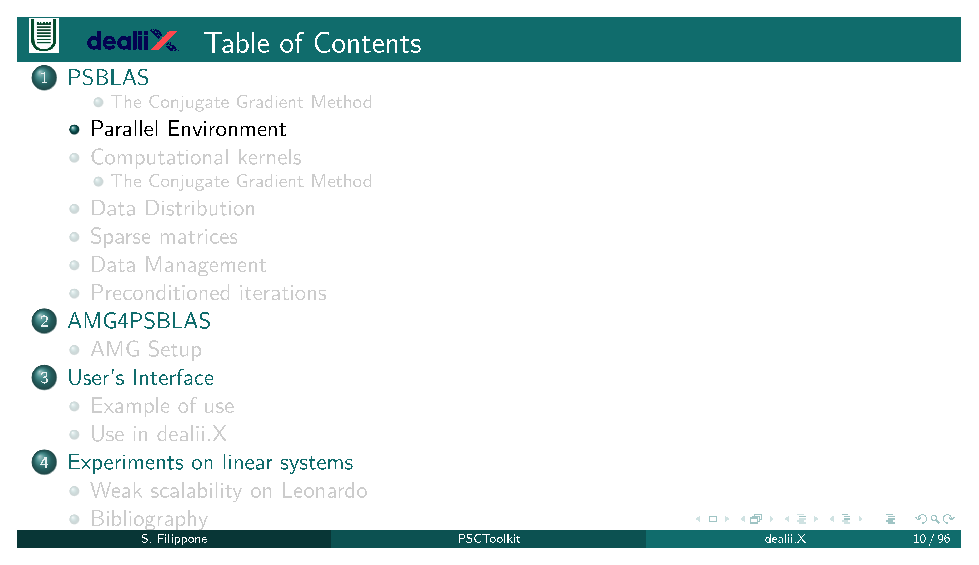
\includegraphics[width=.95\textwidth]{tutorial-013.eps}\\[2\baselineskip]
  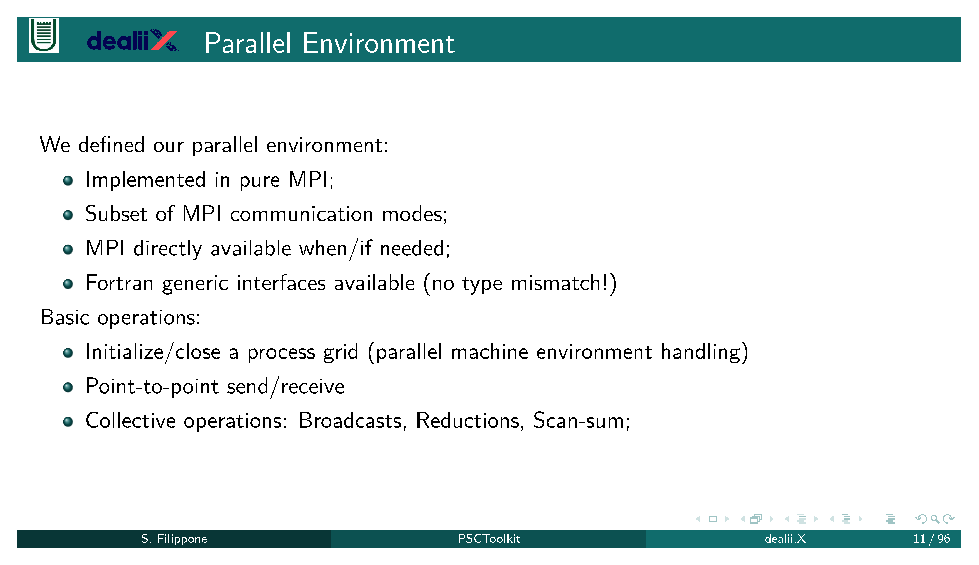
\includegraphics[width=.95\textwidth]{tutorial-014.eps}
\end{center}
\newpage
\begin{center}
  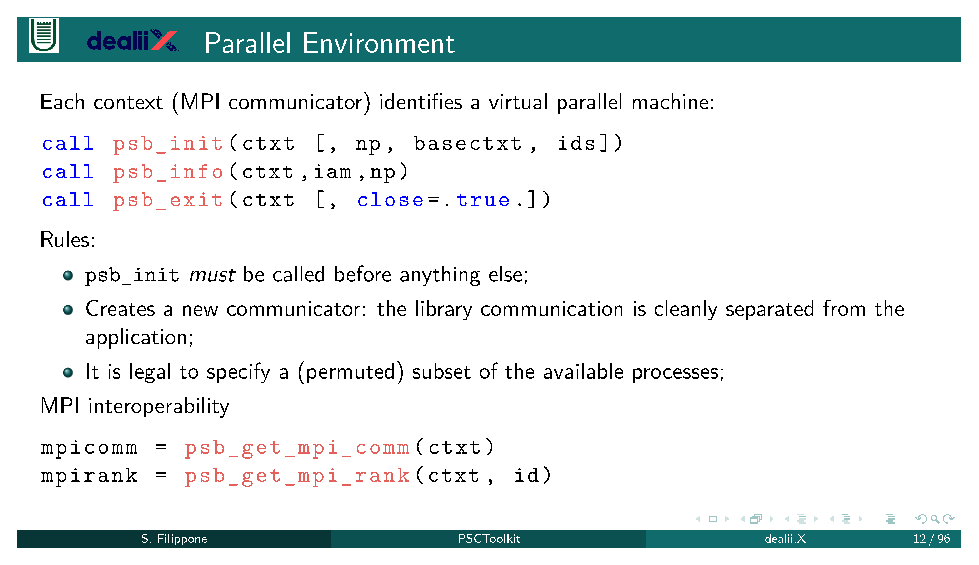
\includegraphics[width=.95\textwidth]{tutorial-015.eps}\\[2\baselineskip]
  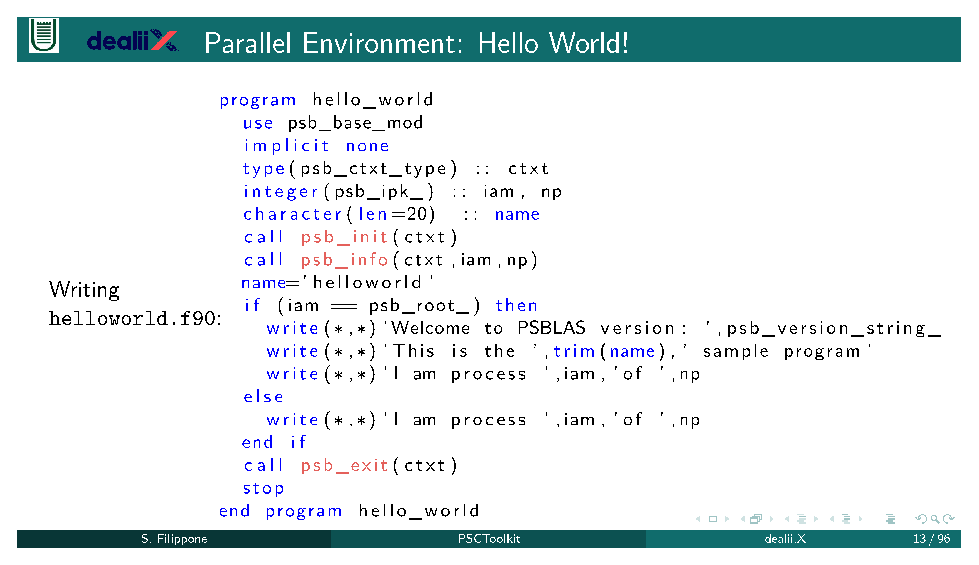
\includegraphics[width=.95\textwidth]{tutorial-016.eps}
\end{center}
\newpage
\begin{center}
  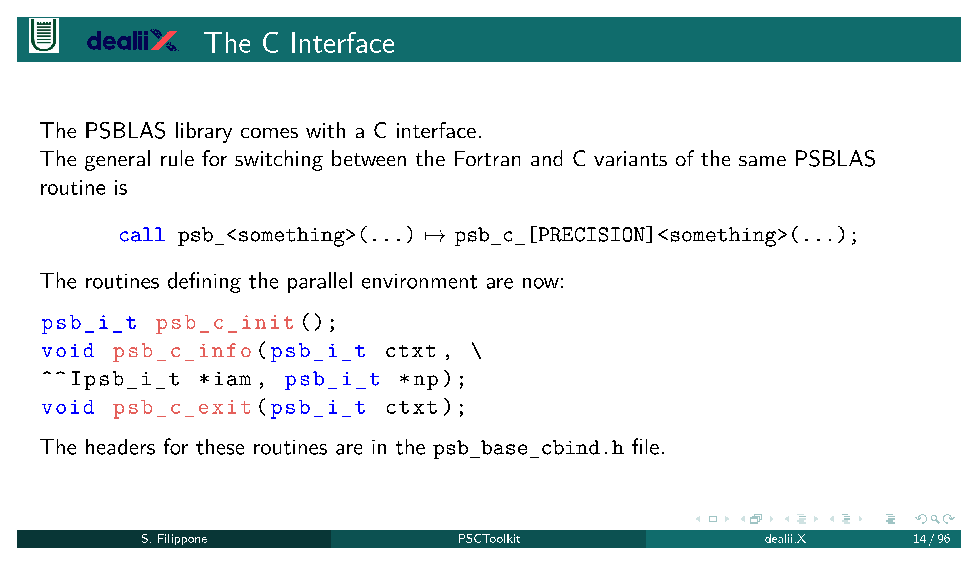
\includegraphics[width=.95\textwidth]{tutorial-017.eps}\\[2\baselineskip]
  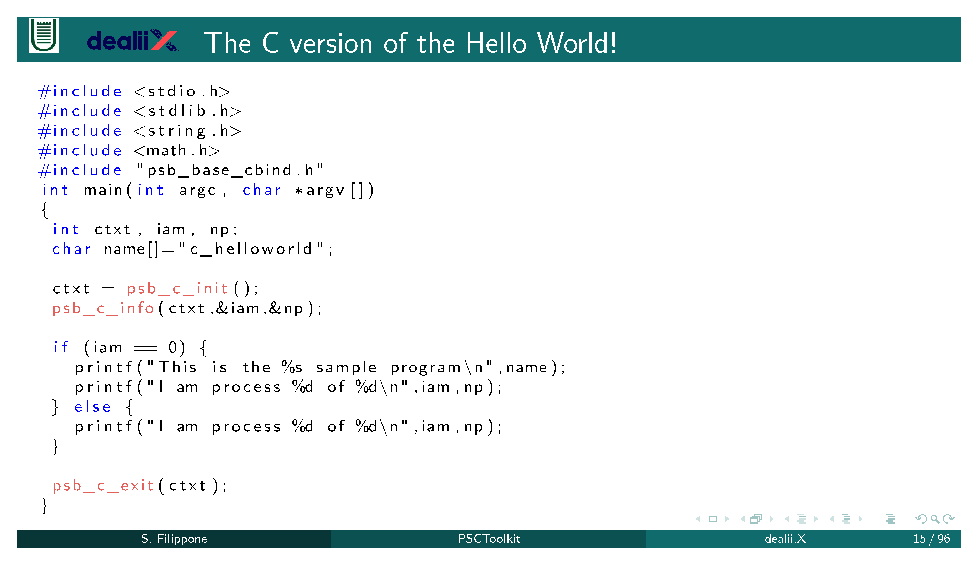
\includegraphics[width=.95\textwidth]{tutorial-018.eps}
\end{center}
\newpage
\begin{center}
  
\includegraphics[width=.95\textwidth]{tutorial-019.eps}\\[2\baselineskip]
  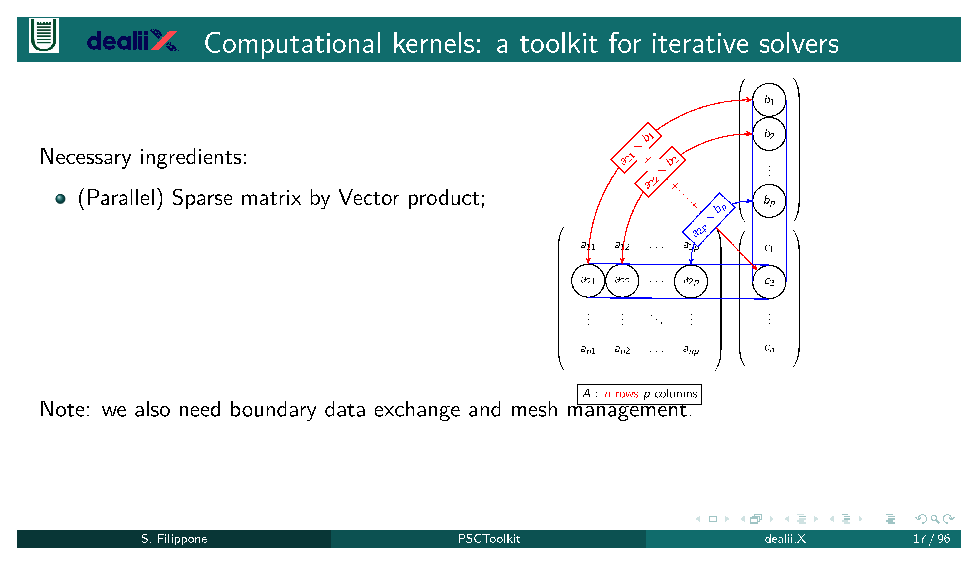
\includegraphics[width=.95\textwidth]{tutorial-020.eps}
\end{center}
\newpage
\begin{center}
  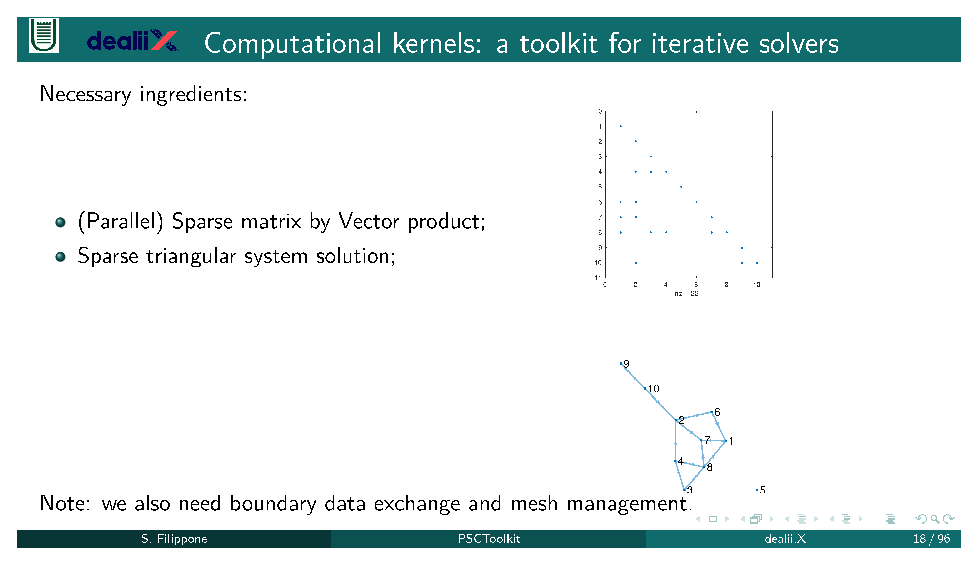
\includegraphics[width=.95\textwidth]{tutorial-021.eps}\\[2\baselineskip]
  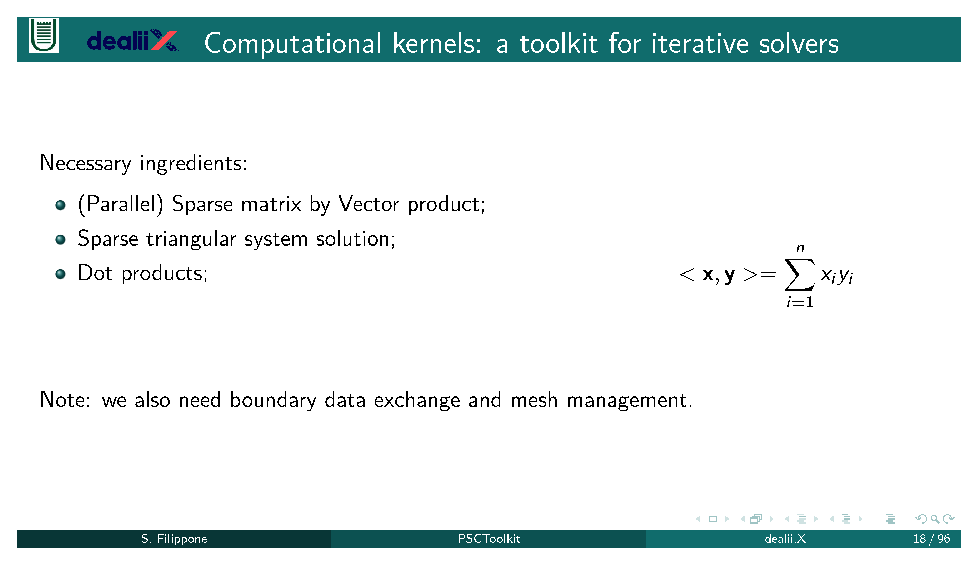
\includegraphics[width=.95\textwidth]{tutorial-022.eps}
\end{center}
\newpage
\begin{center}
  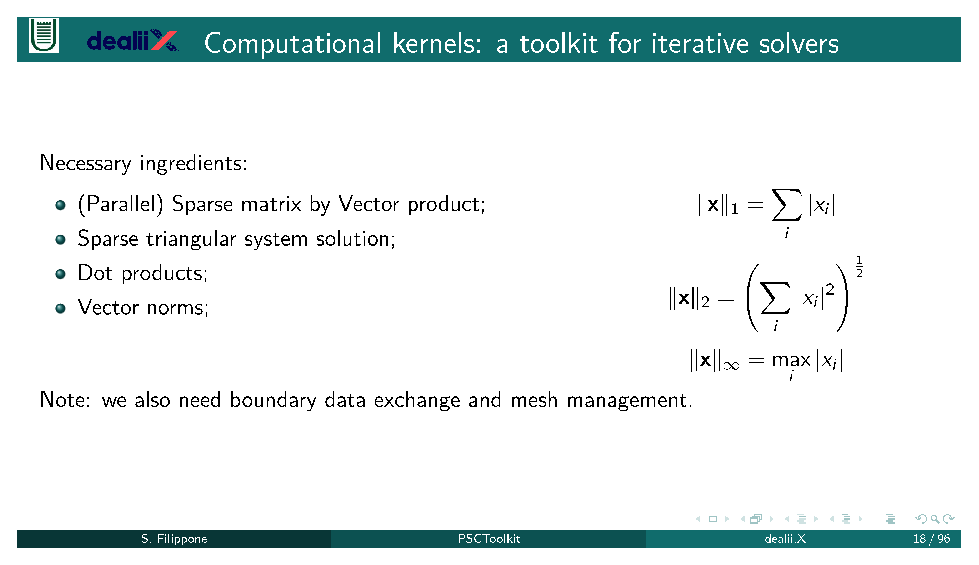
\includegraphics[width=.95\textwidth]{tutorial-023.eps}\\[2\baselineskip]
  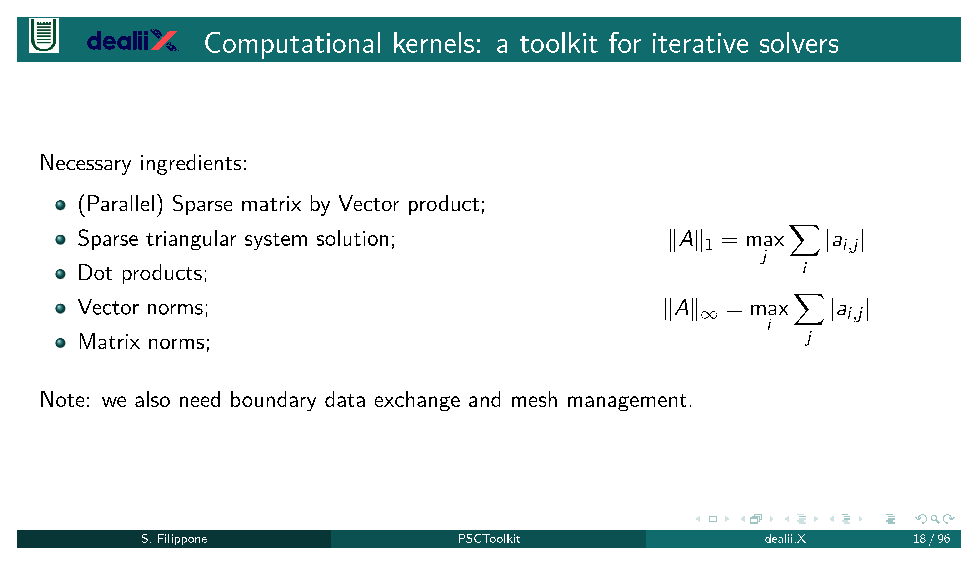
\includegraphics[width=.95\textwidth]{tutorial-024.eps}
\end{center}
\newpage
\begin{center}
  
\includegraphics[width=.95\textwidth]{tutorial-025.eps}\\[2\baselineskip]
  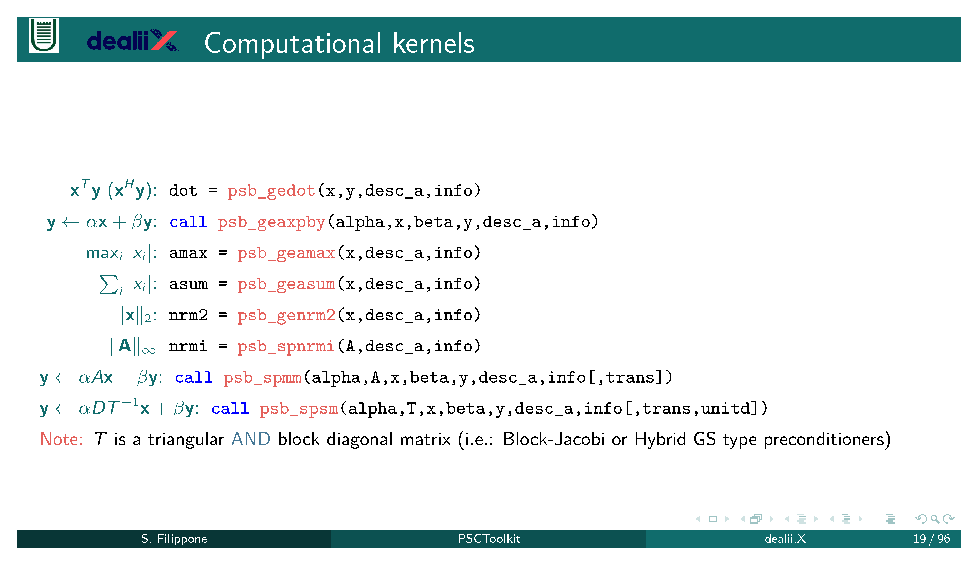
\includegraphics[width=.95\textwidth]{tutorial-026.eps}
\end{center}
\newpage
\begin{center}
  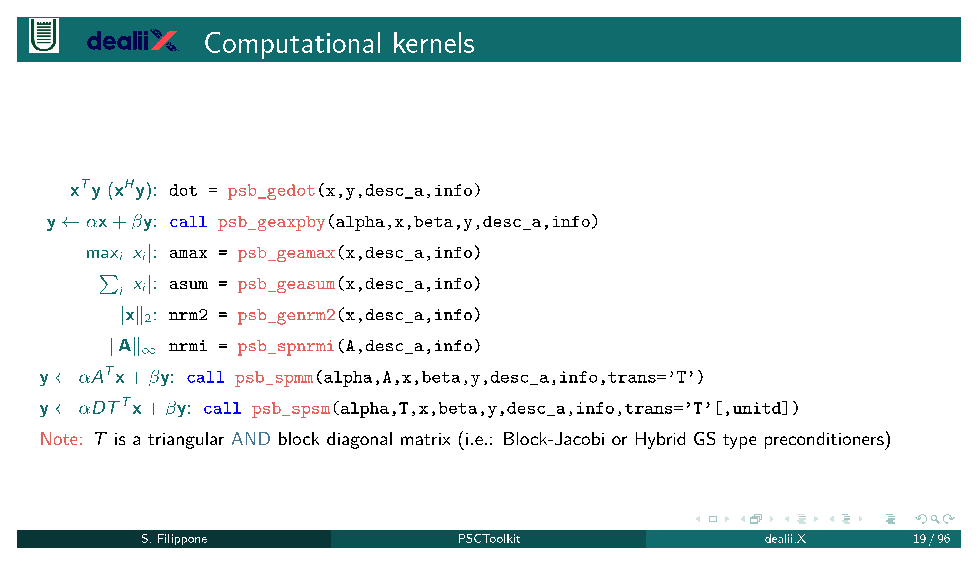
\includegraphics[width=.95\textwidth]{tutorial-027.eps}\\[2\baselineskip]
  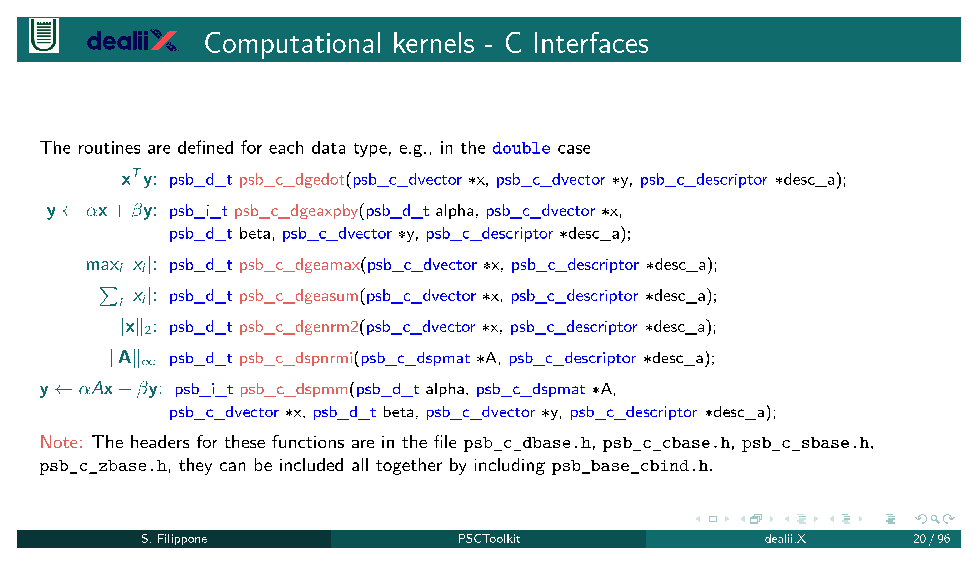
\includegraphics[width=.95\textwidth]{tutorial-028.eps}
\end{center}
\newpage
\begin{center}
  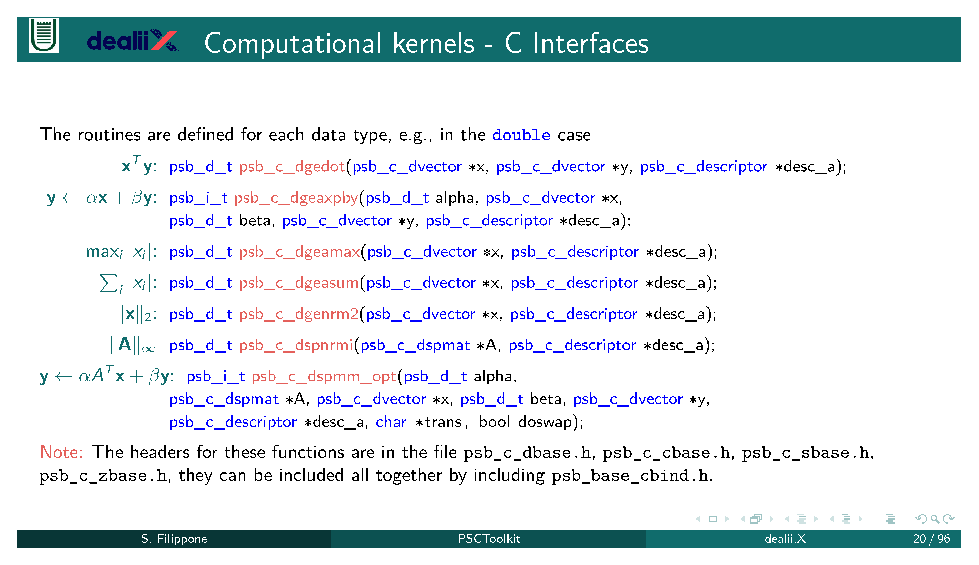
\includegraphics[width=.95\textwidth]{tutorial-029.eps}\\[2\baselineskip]
  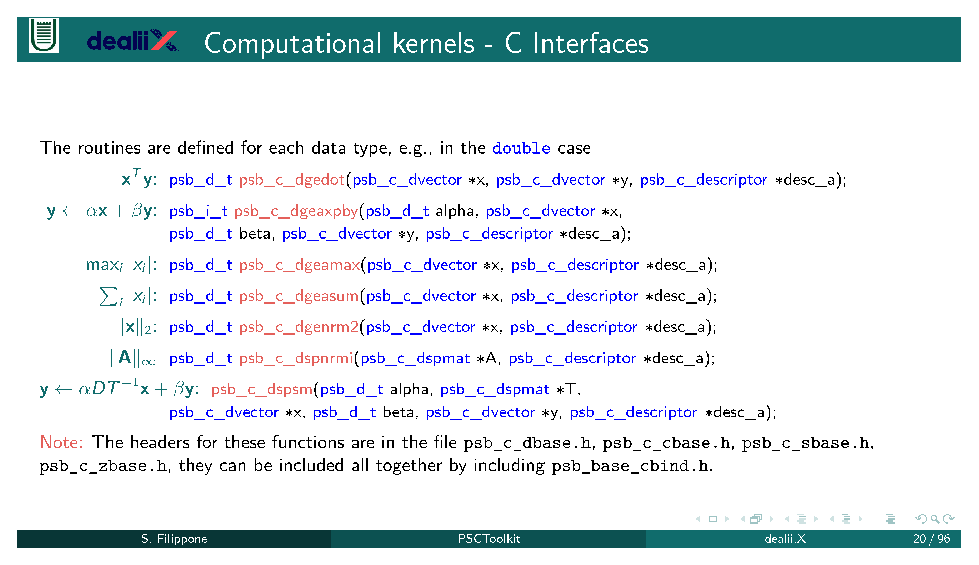
\includegraphics[width=.95\textwidth]{tutorial-030.eps}
\end{center}
\newpage
\begin{center}
  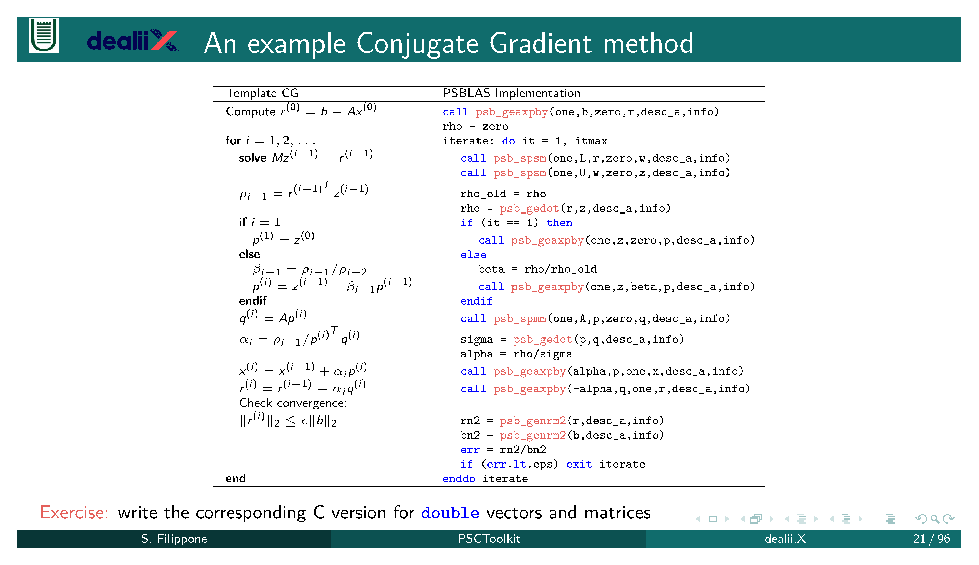
\includegraphics[width=.95\textwidth]{tutorial-031.eps}\\[2\baselineskip]
  
\includegraphics[width=.95\textwidth]{tutorial-032.eps}
\end{center}
\newpage
\begin{center}
  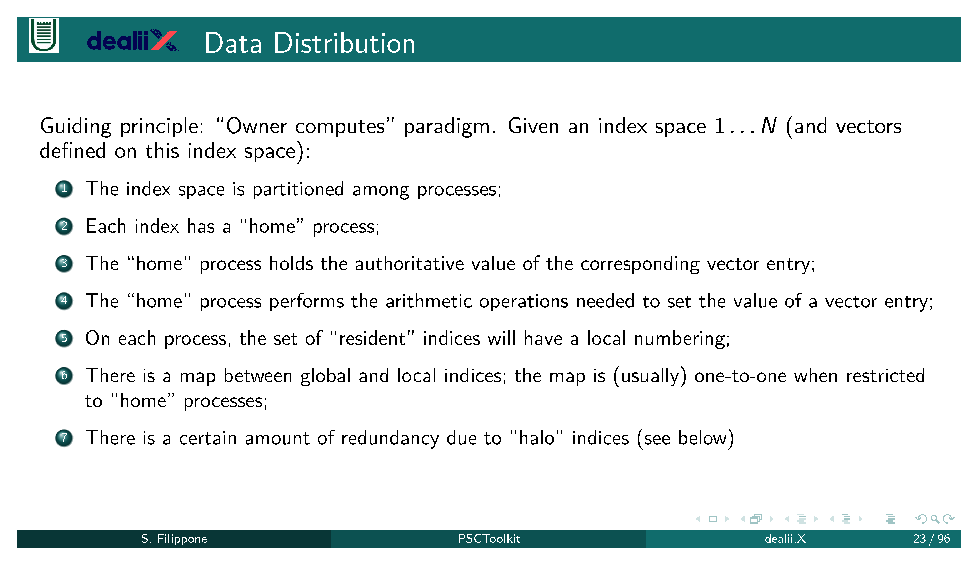
\includegraphics[width=.95\textwidth]{tutorial-033.eps}\\[2\baselineskip]
  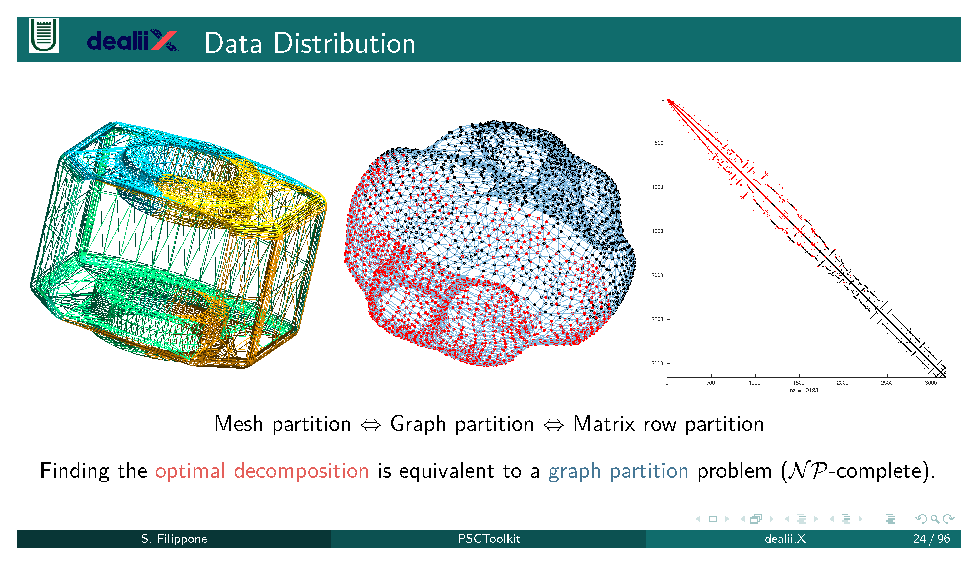
\includegraphics[width=.95\textwidth]{tutorial-034.eps}
\end{center}
\newpage
\begin{center}
  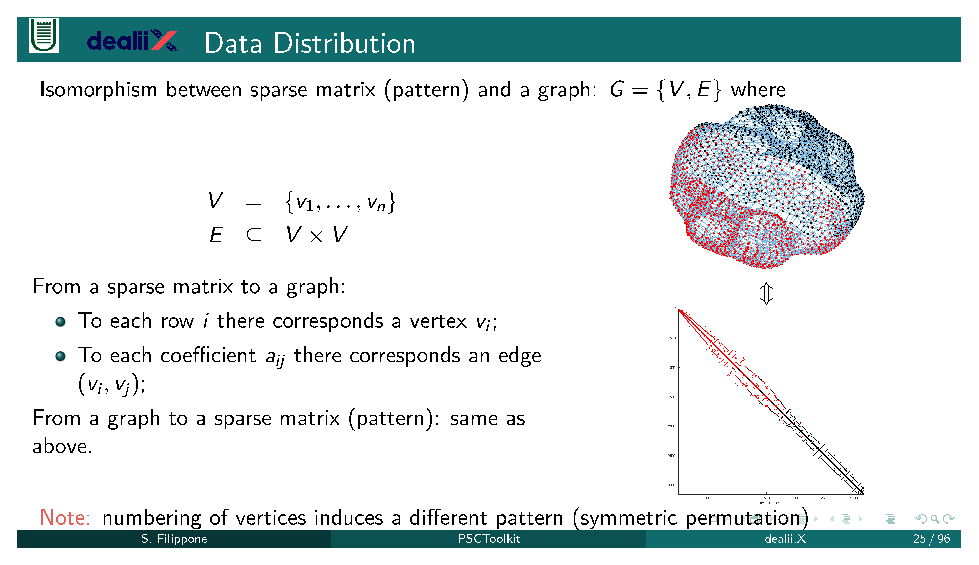
\includegraphics[width=.95\textwidth]{tutorial-035.eps}\\[2\baselineskip]
  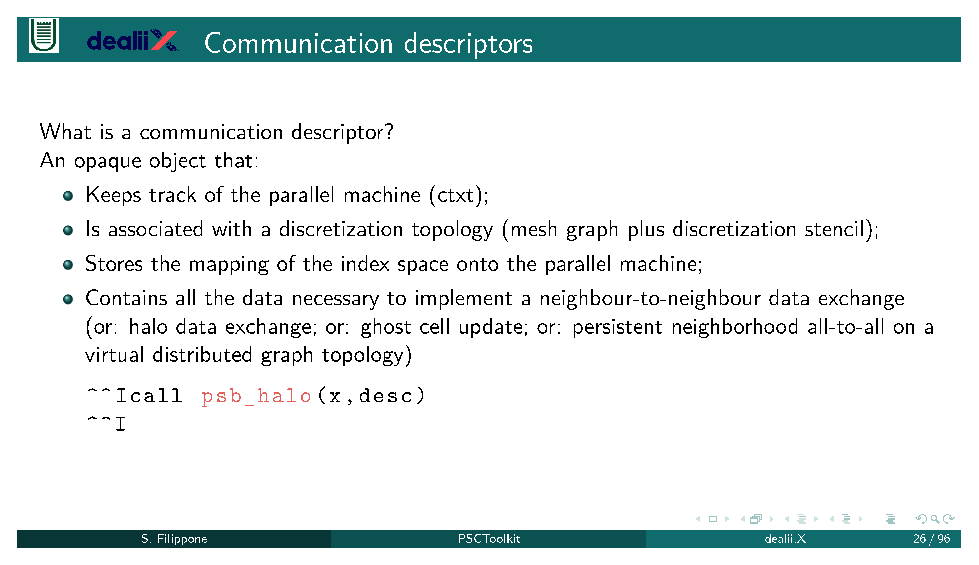
\includegraphics[width=.95\textwidth]{tutorial-036.eps}
\end{center}
\newpage
\begin{center}
  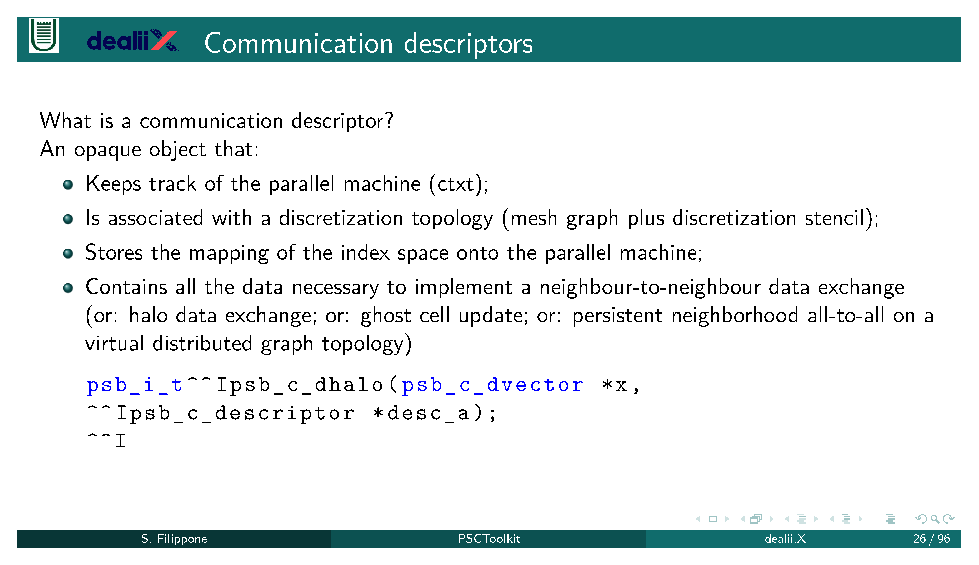
\includegraphics[width=.95\textwidth]{tutorial-037.eps}\\[2\baselineskip]
  
\includegraphics[width=.95\textwidth]{tutorial-038.eps}
\end{center}
\newpage
\begin{center}
  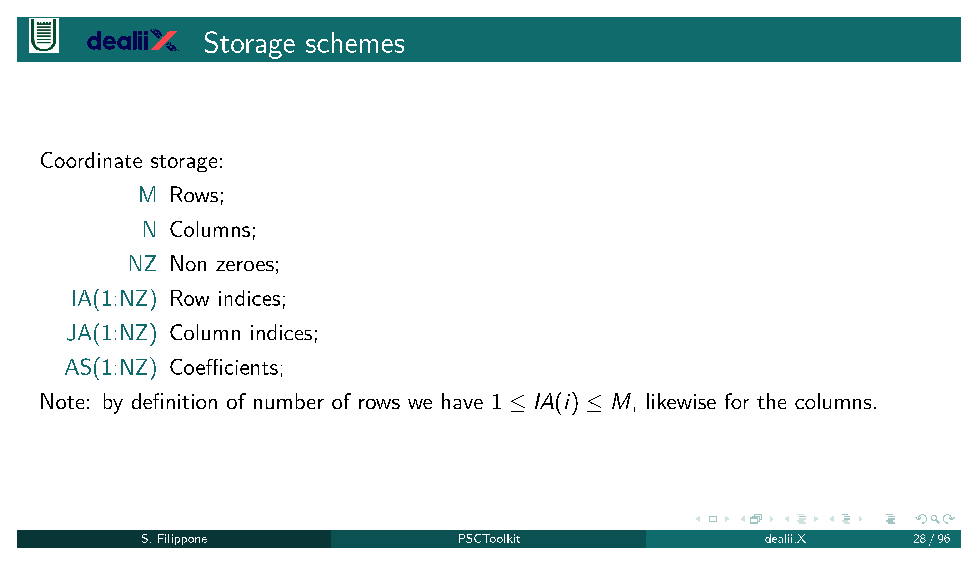
\includegraphics[width=.95\textwidth]{tutorial-039.eps}\\[2\baselineskip]
  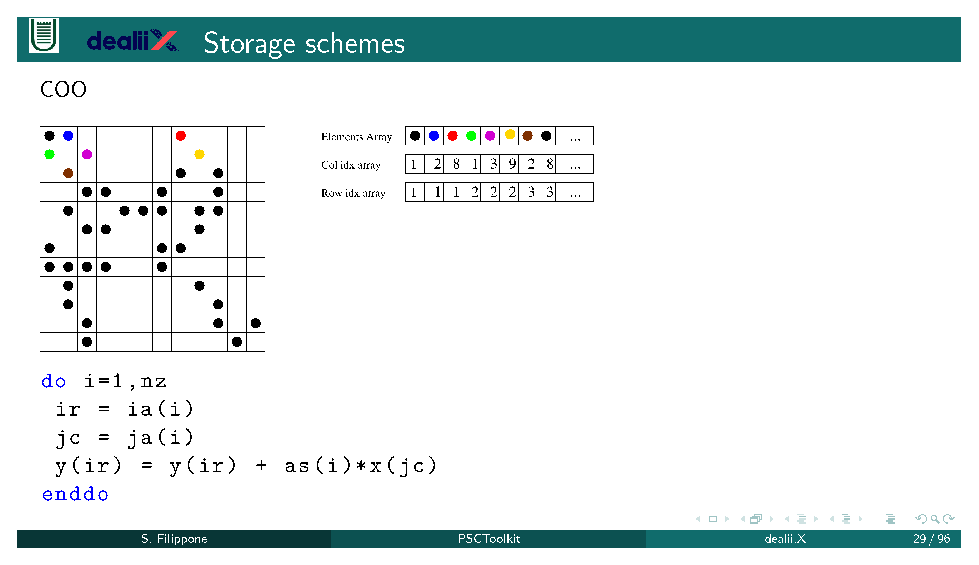
\includegraphics[width=.95\textwidth]{tutorial-040.eps}
\end{center}
\newpage
\begin{center}
  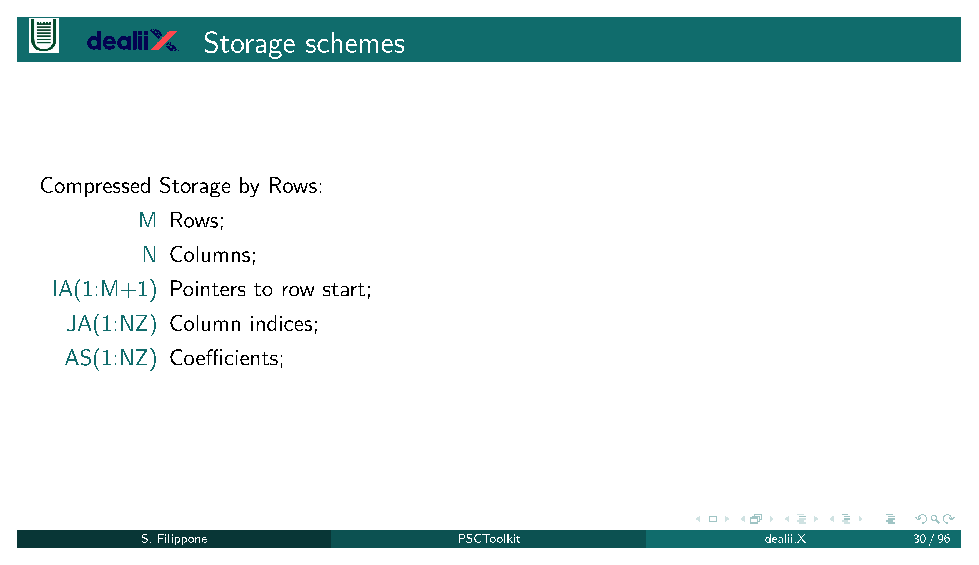
\includegraphics[width=.95\textwidth]{tutorial-041.eps}\\[2\baselineskip]
  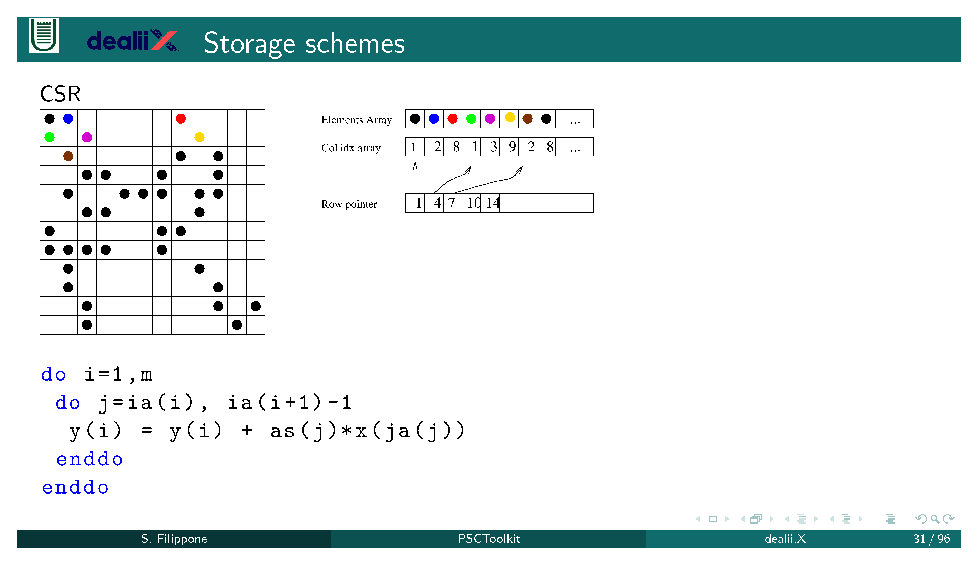
\includegraphics[width=.95\textwidth]{tutorial-042.eps}
\end{center}
\newpage
\begin{center}
  
\includegraphics[width=.95\textwidth]{tutorial-043.eps}\\[2\baselineskip]
  
\includegraphics[width=.95\textwidth]{tutorial-044.eps}
\end{center}
\newpage
\begin{center}
  
\includegraphics[width=.95\textwidth]{tutorial-045.eps}\\[2\baselineskip]
  
\includegraphics[width=.95\textwidth]{tutorial-046.eps}
\end{center}
\newpage
\begin{center}
  
\includegraphics[width=.95\textwidth]{tutorial-047.eps}\\[2\baselineskip]
  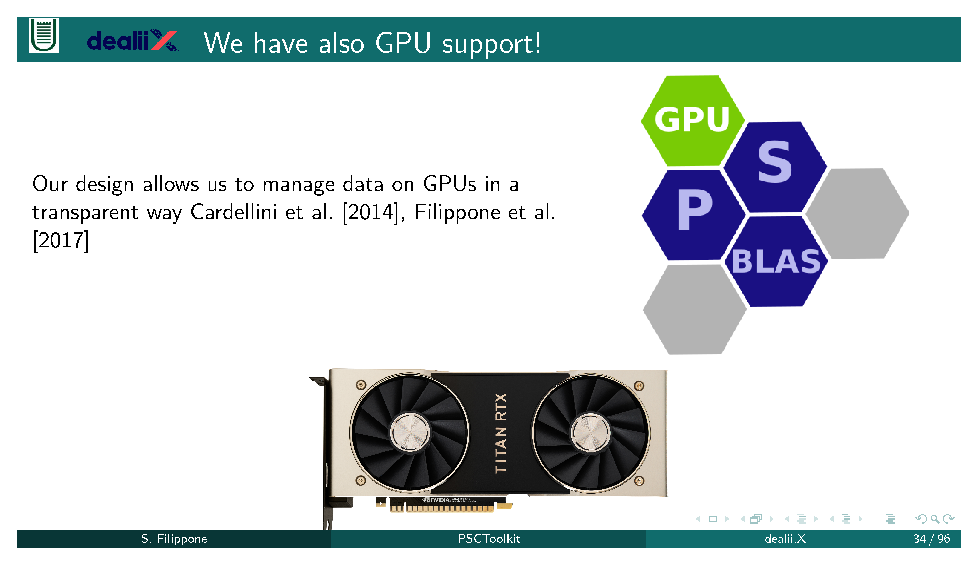
\includegraphics[width=.95\textwidth]{tutorial-048.eps}
\end{center}
\newpage
\begin{center}
  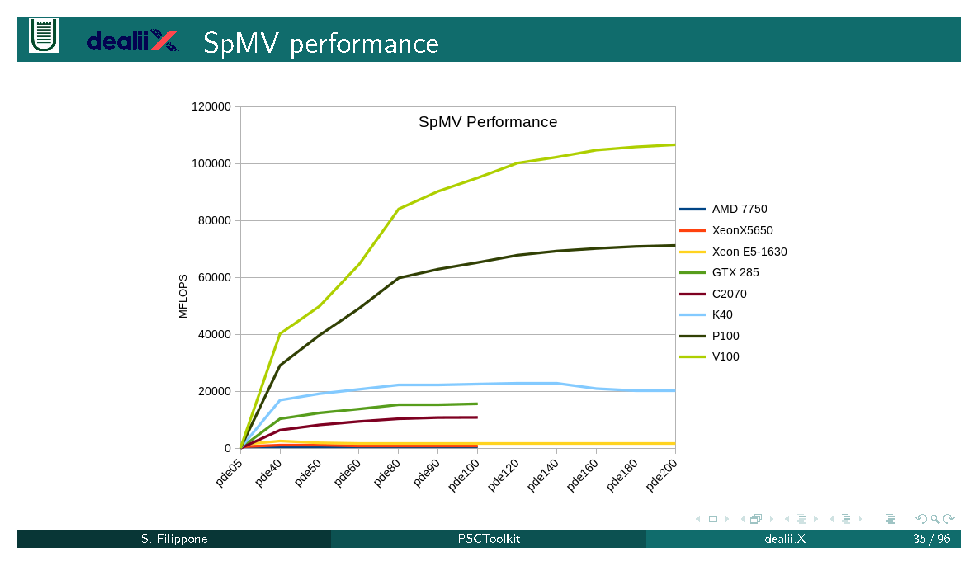
\includegraphics[width=.95\textwidth]{tutorial-049.eps}\\[2\baselineskip]
  
\includegraphics[width=.95\textwidth]{tutorial-050.eps}
\end{center}
\newpage
\begin{center}
  \includegraphics[width=.95\textwidth]{tutorial-051.eps}\\[2\baselineskip]
  \includegraphics[width=.95\textwidth]{tutorial-052.eps}
\end{center}
\newpage
\begin{center}
  \includegraphics[width=.95\textwidth]{tutorial-053.eps}\\[2\baselineskip]
  \includegraphics[width=.95\textwidth]{tutorial-054.eps}
\end{center}
\newpage
\begin{center}
  \includegraphics[width=.95\textwidth]{tutorial-055.eps}\\[2\baselineskip]
  \includegraphics[width=.95\textwidth]{tutorial-056.eps}
\end{center}
\newpage
\begin{center}
  \includegraphics[width=.95\textwidth]{tutorial-057.eps}\\[2\baselineskip]
  \includegraphics[width=.95\textwidth]{tutorial-058.eps}
\end{center}
\newpage
\begin{center}
  \includegraphics[width=.95\textwidth]{tutorial-059.eps}\\[2\baselineskip]
  \includegraphics[width=.95\textwidth]{tutorial-060.eps}
\end{center}
\newpage
\begin{center}
  \includegraphics[width=.95\textwidth]{tutorial-061.eps}\\[2\baselineskip]
  \includegraphics[width=.95\textwidth]{tutorial-062.eps}
\end{center}
\newpage
\begin{center}
  \includegraphics[width=.95\textwidth]{tutorial-063.eps}\\[2\baselineskip]
  \includegraphics[width=.95\textwidth]{tutorial-064.eps}
\end{center}
\newpage
\begin{center}
  \includegraphics[width=.95\textwidth]{tutorial-065.eps}\\[2\baselineskip]
  \includegraphics[width=.95\textwidth]{tutorial-066.eps}
\end{center}
\newpage
\begin{center}
  \includegraphics[width=.95\textwidth]{tutorial-067.eps}\\[2\baselineskip]
  \includegraphics[width=.95\textwidth]{tutorial-068.eps}
\end{center}
\newpage
\begin{center}
  \includegraphics[width=.95\textwidth]{tutorial-069.eps}\\[2\baselineskip]
  \includegraphics[width=.95\textwidth]{tutorial-070.eps}
\end{center}
\newpage
\begin{center}
  \includegraphics[width=.95\textwidth]{tutorial-071.eps}\\[2\baselineskip]
  \includegraphics[width=.95\textwidth]{tutorial-072.eps}
\end{center}
\newpage
\begin{center}
  \includegraphics[width=.95\textwidth]{tutorial-073.eps}\\[2\baselineskip]
  \includegraphics[width=.95\textwidth]{tutorial-074.eps}
\end{center}
\newpage
\begin{center}
  \includegraphics[width=.95\textwidth]{tutorial-075.eps}\\[2\baselineskip]
  \includegraphics[width=.95\textwidth]{tutorial-076.eps}
\end{center}
\newpage
\begin{center}
  \includegraphics[width=.95\textwidth]{tutorial-077.eps}\\[2\baselineskip]
  \includegraphics[width=.95\textwidth]{tutorial-078.eps}
\end{center}
\newpage
\begin{center}
  \includegraphics[width=.95\textwidth]{tutorial-079.eps}\\[2\baselineskip]
  \includegraphics[width=.95\textwidth]{tutorial-080.eps}
\end{center}
\newpage
\begin{center}
  \includegraphics[width=.95\textwidth]{tutorial-081.eps}\\[2\baselineskip]
  \includegraphics[width=.95\textwidth]{tutorial-082.eps}
\end{center}
\newpage
\begin{center}
  \includegraphics[width=.95\textwidth]{tutorial-083.eps}\\[2\baselineskip]
  \includegraphics[width=.95\textwidth]{tutorial-084.eps}
\end{center}
\newpage
\begin{center}
  \includegraphics[width=.95\textwidth]{tutorial-085.eps}\\[2\baselineskip]
  \includegraphics[width=.95\textwidth]{tutorial-086.eps}
\end{center}
\newpage
\begin{center}
  \includegraphics[width=.95\textwidth]{tutorial-087.eps}\\[2\baselineskip]
  \includegraphics[width=.95\textwidth]{tutorial-088.eps}
\end{center}
\newpage
\begin{center}
  \includegraphics[width=.95\textwidth]{tutorial-089.eps}\\[2\baselineskip]
  \includegraphics[width=.95\textwidth]{tutorial-090.eps}
\end{center}
\newpage
\begin{center}
  \includegraphics[width=.95\textwidth]{tutorial-091.eps}\\[2\baselineskip]
  \includegraphics[width=.95\textwidth]{tutorial-092.eps}
\end{center}
\newpage
\begin{center}
  \includegraphics[width=.95\textwidth]{tutorial-093.eps}\\[2\baselineskip]
  \includegraphics[width=.95\textwidth]{tutorial-094.eps}
\end{center}
\newpage
\begin{center}
  \includegraphics[width=.95\textwidth]{tutorial-095.eps}\\[2\baselineskip]
  \includegraphics[width=.95\textwidth]{tutorial-096.eps}
\end{center}
\newpage
\begin{center}
  \includegraphics[width=.95\textwidth]{tutorial-097.eps}\\[2\baselineskip]
  \includegraphics[width=.95\textwidth]{tutorial-098.eps}
\end{center}
\newpage
\begin{center}
  \includegraphics[width=.95\textwidth]{tutorial-099.eps}\\[2\baselineskip]
  \includegraphics[width=.95\textwidth]{tutorial-100.eps}
\end{center}
\newpage
\begin{center}
  \includegraphics[width=.95\textwidth]{tutorial-101.eps}\\[2\baselineskip]
  \includegraphics[width=.95\textwidth]{tutorial-102.eps}
\end{center}
\newpage
\begin{center}
  \includegraphics[width=.95\textwidth]{tutorial-103.eps}\\[2\baselineskip]
  \includegraphics[width=.95\textwidth]{tutorial-104.eps}
\end{center}
\newpage
\begin{center}
  \includegraphics[width=.95\textwidth]{tutorial-105.eps}\\[2\baselineskip]
  \includegraphics[width=.95\textwidth]{tutorial-106.eps}
\end{center}
\newpage
\begin{center}
  \includegraphics[width=.95\textwidth]{tutorial-107.eps}\\[2\baselineskip]
  \includegraphics[width=.95\textwidth]{tutorial-108.eps}
\end{center}
\newpage
\begin{center}
  \includegraphics[width=.95\textwidth]{tutorial-109.eps}\\[2\baselineskip]
  \includegraphics[width=.95\textwidth]{tutorial-110.eps}
\end{center}
\newpage
\begin{center}
  \includegraphics[width=.95\textwidth]{tutorial-111.eps}\\[2\baselineskip]
  \includegraphics[width=.95\textwidth]{tutorial-112.eps}
\end{center}
\newpage
\begin{center}
  \includegraphics[width=.95\textwidth]{tutorial-113.eps}\\[2\baselineskip]
  \includegraphics[width=.95\textwidth]{tutorial-114.eps}
\end{center}
\newpage
\begin{center}
  \includegraphics[width=.95\textwidth]{tutorial-115.eps}\\[2\baselineskip]
  \includegraphics[width=.95\textwidth]{tutorial-116.eps}
\end{center}
\newpage
\begin{center}
  \includegraphics[width=.95\textwidth]{tutorial-117.eps}\\[2\baselineskip]
  \includegraphics[width=.95\textwidth]{tutorial-118.eps}
\end{center}
\newpage
\begin{center}
  \includegraphics[width=.95\textwidth]{tutorial-119.eps}\\[2\baselineskip]
  \includegraphics[width=.95\textwidth]{tutorial-120.eps}
\end{center}
\newpage
\begin{center}
  \includegraphics[width=.95\textwidth]{tutorial-121.eps}\\[2\baselineskip]
  \includegraphics[width=.95\textwidth]{tutorial-122.eps}
\end{center}
\newpage
\begin{center}
  \includegraphics[width=.95\textwidth]{tutorial-123.eps}\\[2\baselineskip]
  \includegraphics[width=.95\textwidth]{tutorial-124.eps}
\end{center}
\newpage
\begin{center}
  \includegraphics[width=.95\textwidth]{tutorial-125.eps}\\[2\baselineskip]
  \includegraphics[width=.95\textwidth]{tutorial-126.eps}
\end{center}
\newpage



\subsection{{[Subsection Title]}}

\subsection{{[Subsection Title]}}

\newpage

\section{{[Section Title]}}
\label{sec:section3}


\subsection{{[Subsection Title]}}
\begin{itemize}[left=1em, itemsep=0pt, topsep=0pt] 
    \item 
    \item 
    \item 
\end{itemize}

\subsection{{[Subsection Title]}}

\newpage

\section{{[Section Title]}}
\label{sec:section4}


\begin{center}
    \begin{table}[h!]
    \small
    \caption{[Table Caption]}
    \renewcommand{\arraystretch}{1.25}
    \label{tab:example_table}
    \begin{tabular}{|l|l|l|c|}
    \hline
    \textbf{Column 1} & \textbf{Column 2} & \textbf{Column 3} & \textbf{Column 4} \\
    \hline
    Item 1 & Description & Category & Value \\
    Item 2 & Description & Category & Value \\
    Item 3 & Description & Category & Value \\
    \hline
    \end{tabular}
    \end{table}
\end{center}

\newpage

\section{{[Section Title]}}
\label{sec:section5}


\subsection{{[Subsection Title]}}

\subsection{{[Subsection Title]}}
\begin{itemize}[left=1em, itemsep=0pt, topsep=0pt] 
    \item \textbf{[Item Title]}: 
    \item \textbf{[Item Title]}: 
    \item \textbf{[Item Title]}: 
\end{itemize}

\newpage

\section{{[Section Title]}}
\label{sec:section6}


\begin{center}
\resizebox{\textwidth}{!}{
\begin{tabular}{|l|l|l|}
\hline
\textbf{Column 1} & \textbf{Column 2} & \textbf{Column 3} \\
\hline
Item 1 & Description & Value \\
\hline
Item 2 & Description & Value \\
\hline
Item 3 & Description & Value \\
\hline
\end{tabular}}
\label{tab:example_table2}
\end{center}

\newpage 

\section{{Conclusion}} \label{sec:conclusion}


\label{MyLastPage}

\end{document}
